\section{Appendix}

\subsection{Sample Description}

% latex table generated in R 3.1.3 by xtable 1.7-4 package
% Thu Apr  2 14:31:00 2015
\begin{table}[ht]
\centering
\begin{tabular}{lrrrr}
  \hline
 & Group 1 & Group 2 & Difference & p-value \\ 
  \hline
  Self & 38.470 & 39.619 & -1.149 & 0.614 \\ 
  Party & 41.606 & 42.167 & -0.562 & 0.810 \\ 
  Self (Democrats) & 25.265 & 27.031 & -1.767 & 0.373 \\ 
  Self (Republican) & 68.255 & 70.386 & -2.131 & 0.517 \\ 
  Party (Democrats) & 28.290 & 27.637 & 0.653 & 0.723 \\ 
  Party (Republican) & 75.764 & 78.737 & -2.973 & 0.352 \\ 
   \hline
\end{tabular}
\caption{Means for self and party placement in both groups for both experiments and split by preferred party. p-values from 2 sided difference in means tests.} 
\label{tab:means}
\end{table}


\begin{figure}[ht!]
  \centering
  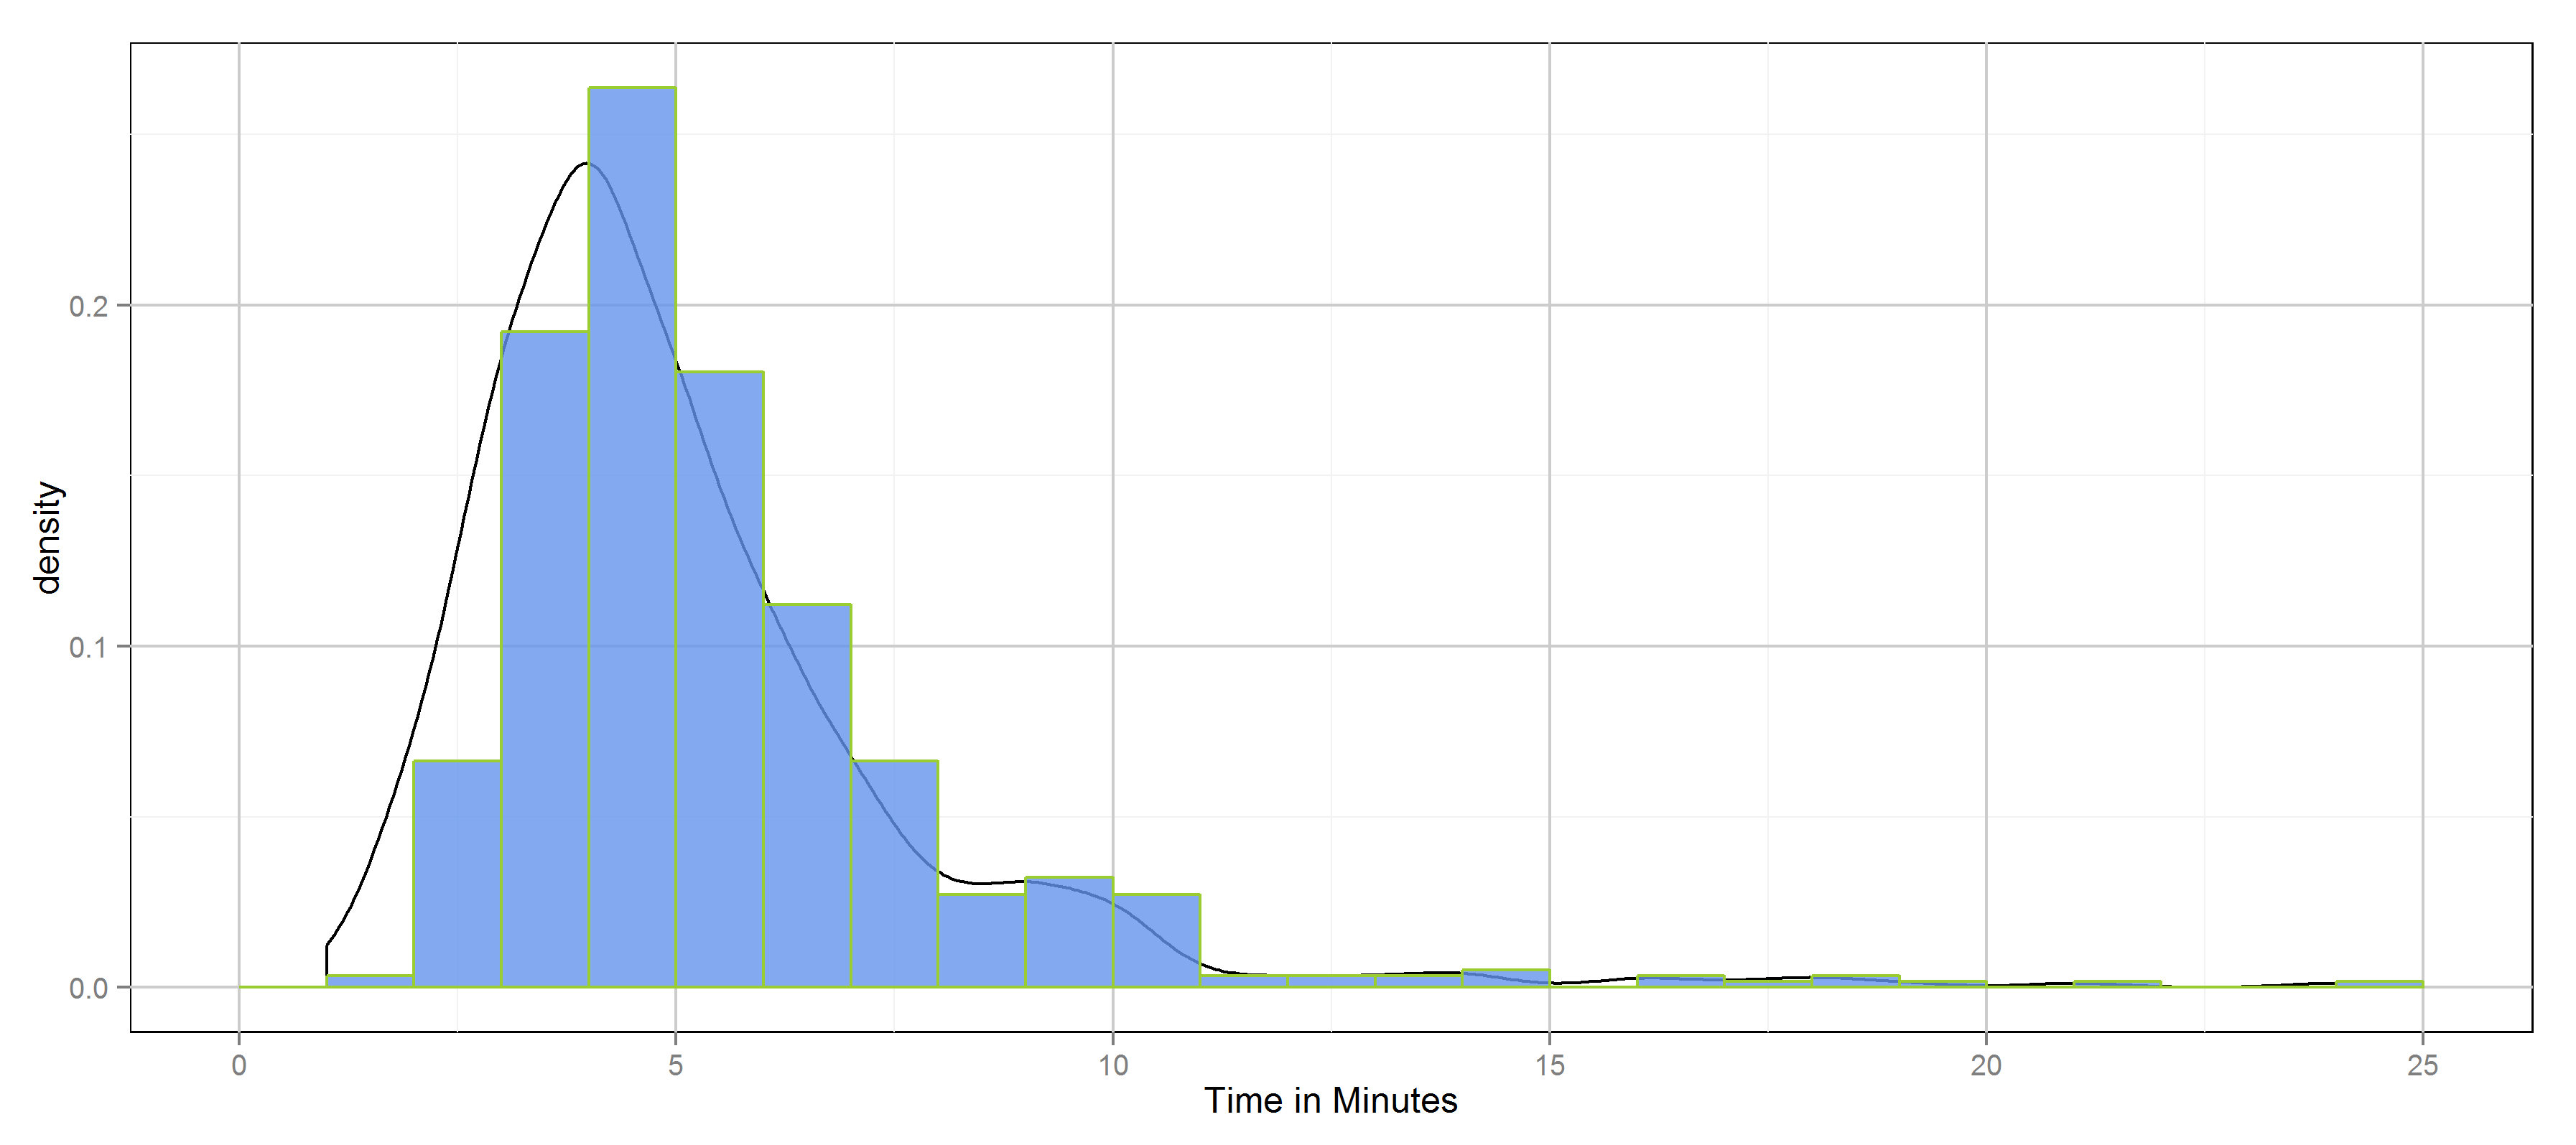
\includegraphics{../figures/main/time.png}
  \caption{Distribution of time in minutes respondents needed to complete the survey.}
  \label{fig:time}
\end{figure}

\begin{figure}[ht!]
  \centering
  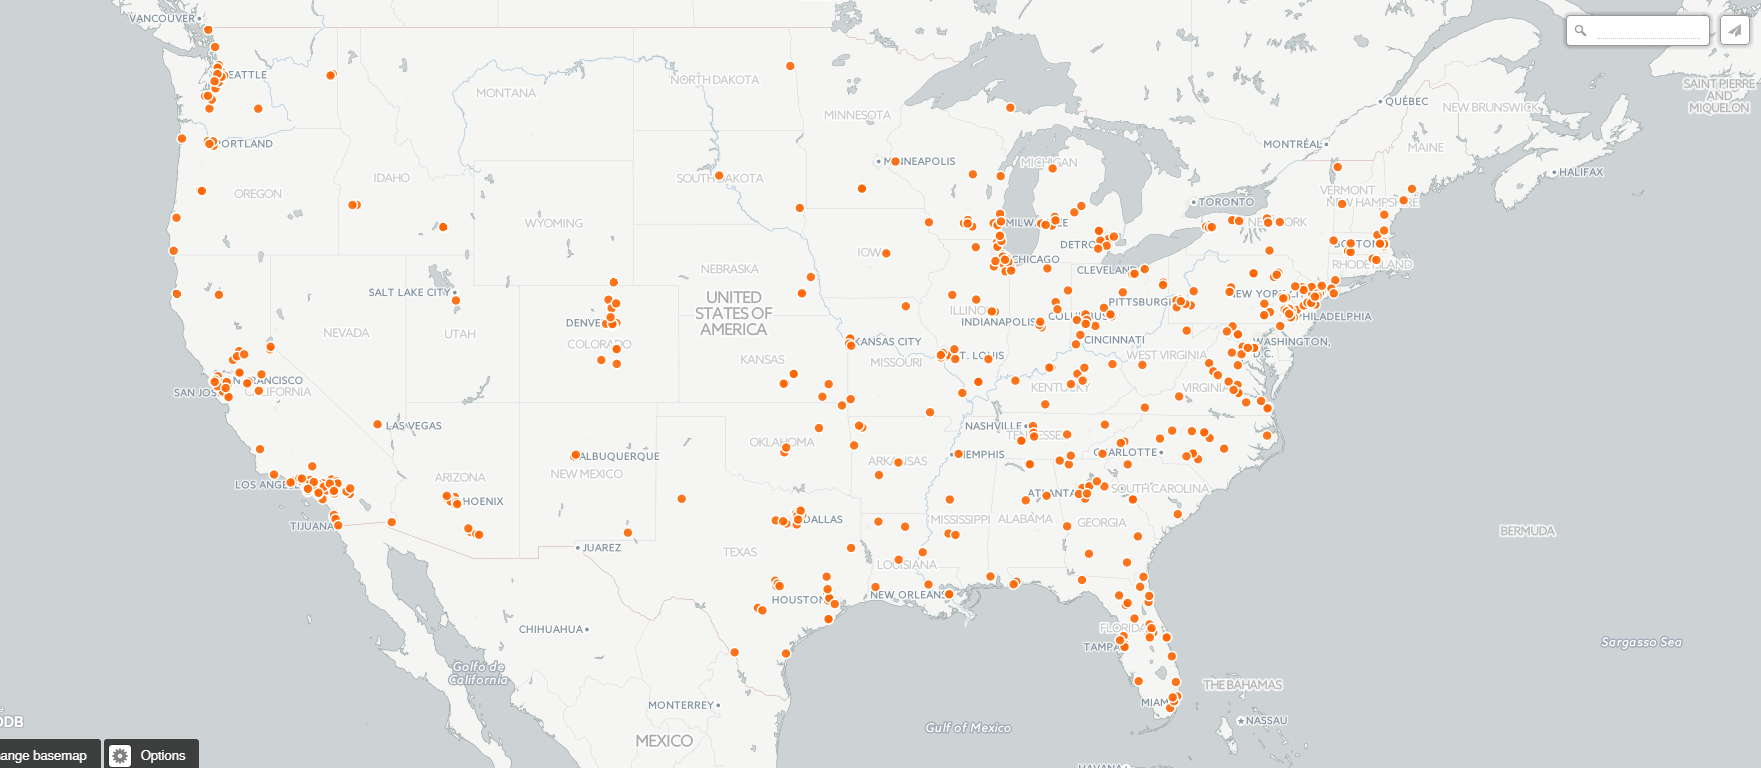
\includegraphics{../figures/main/us_map.png}
  \caption{Geographical distribution of respondents (respondents with ip addresses outside the US removed).}
  \label{fig:map}
\end{figure}

\begin{figure}[ht!]
  \centering
  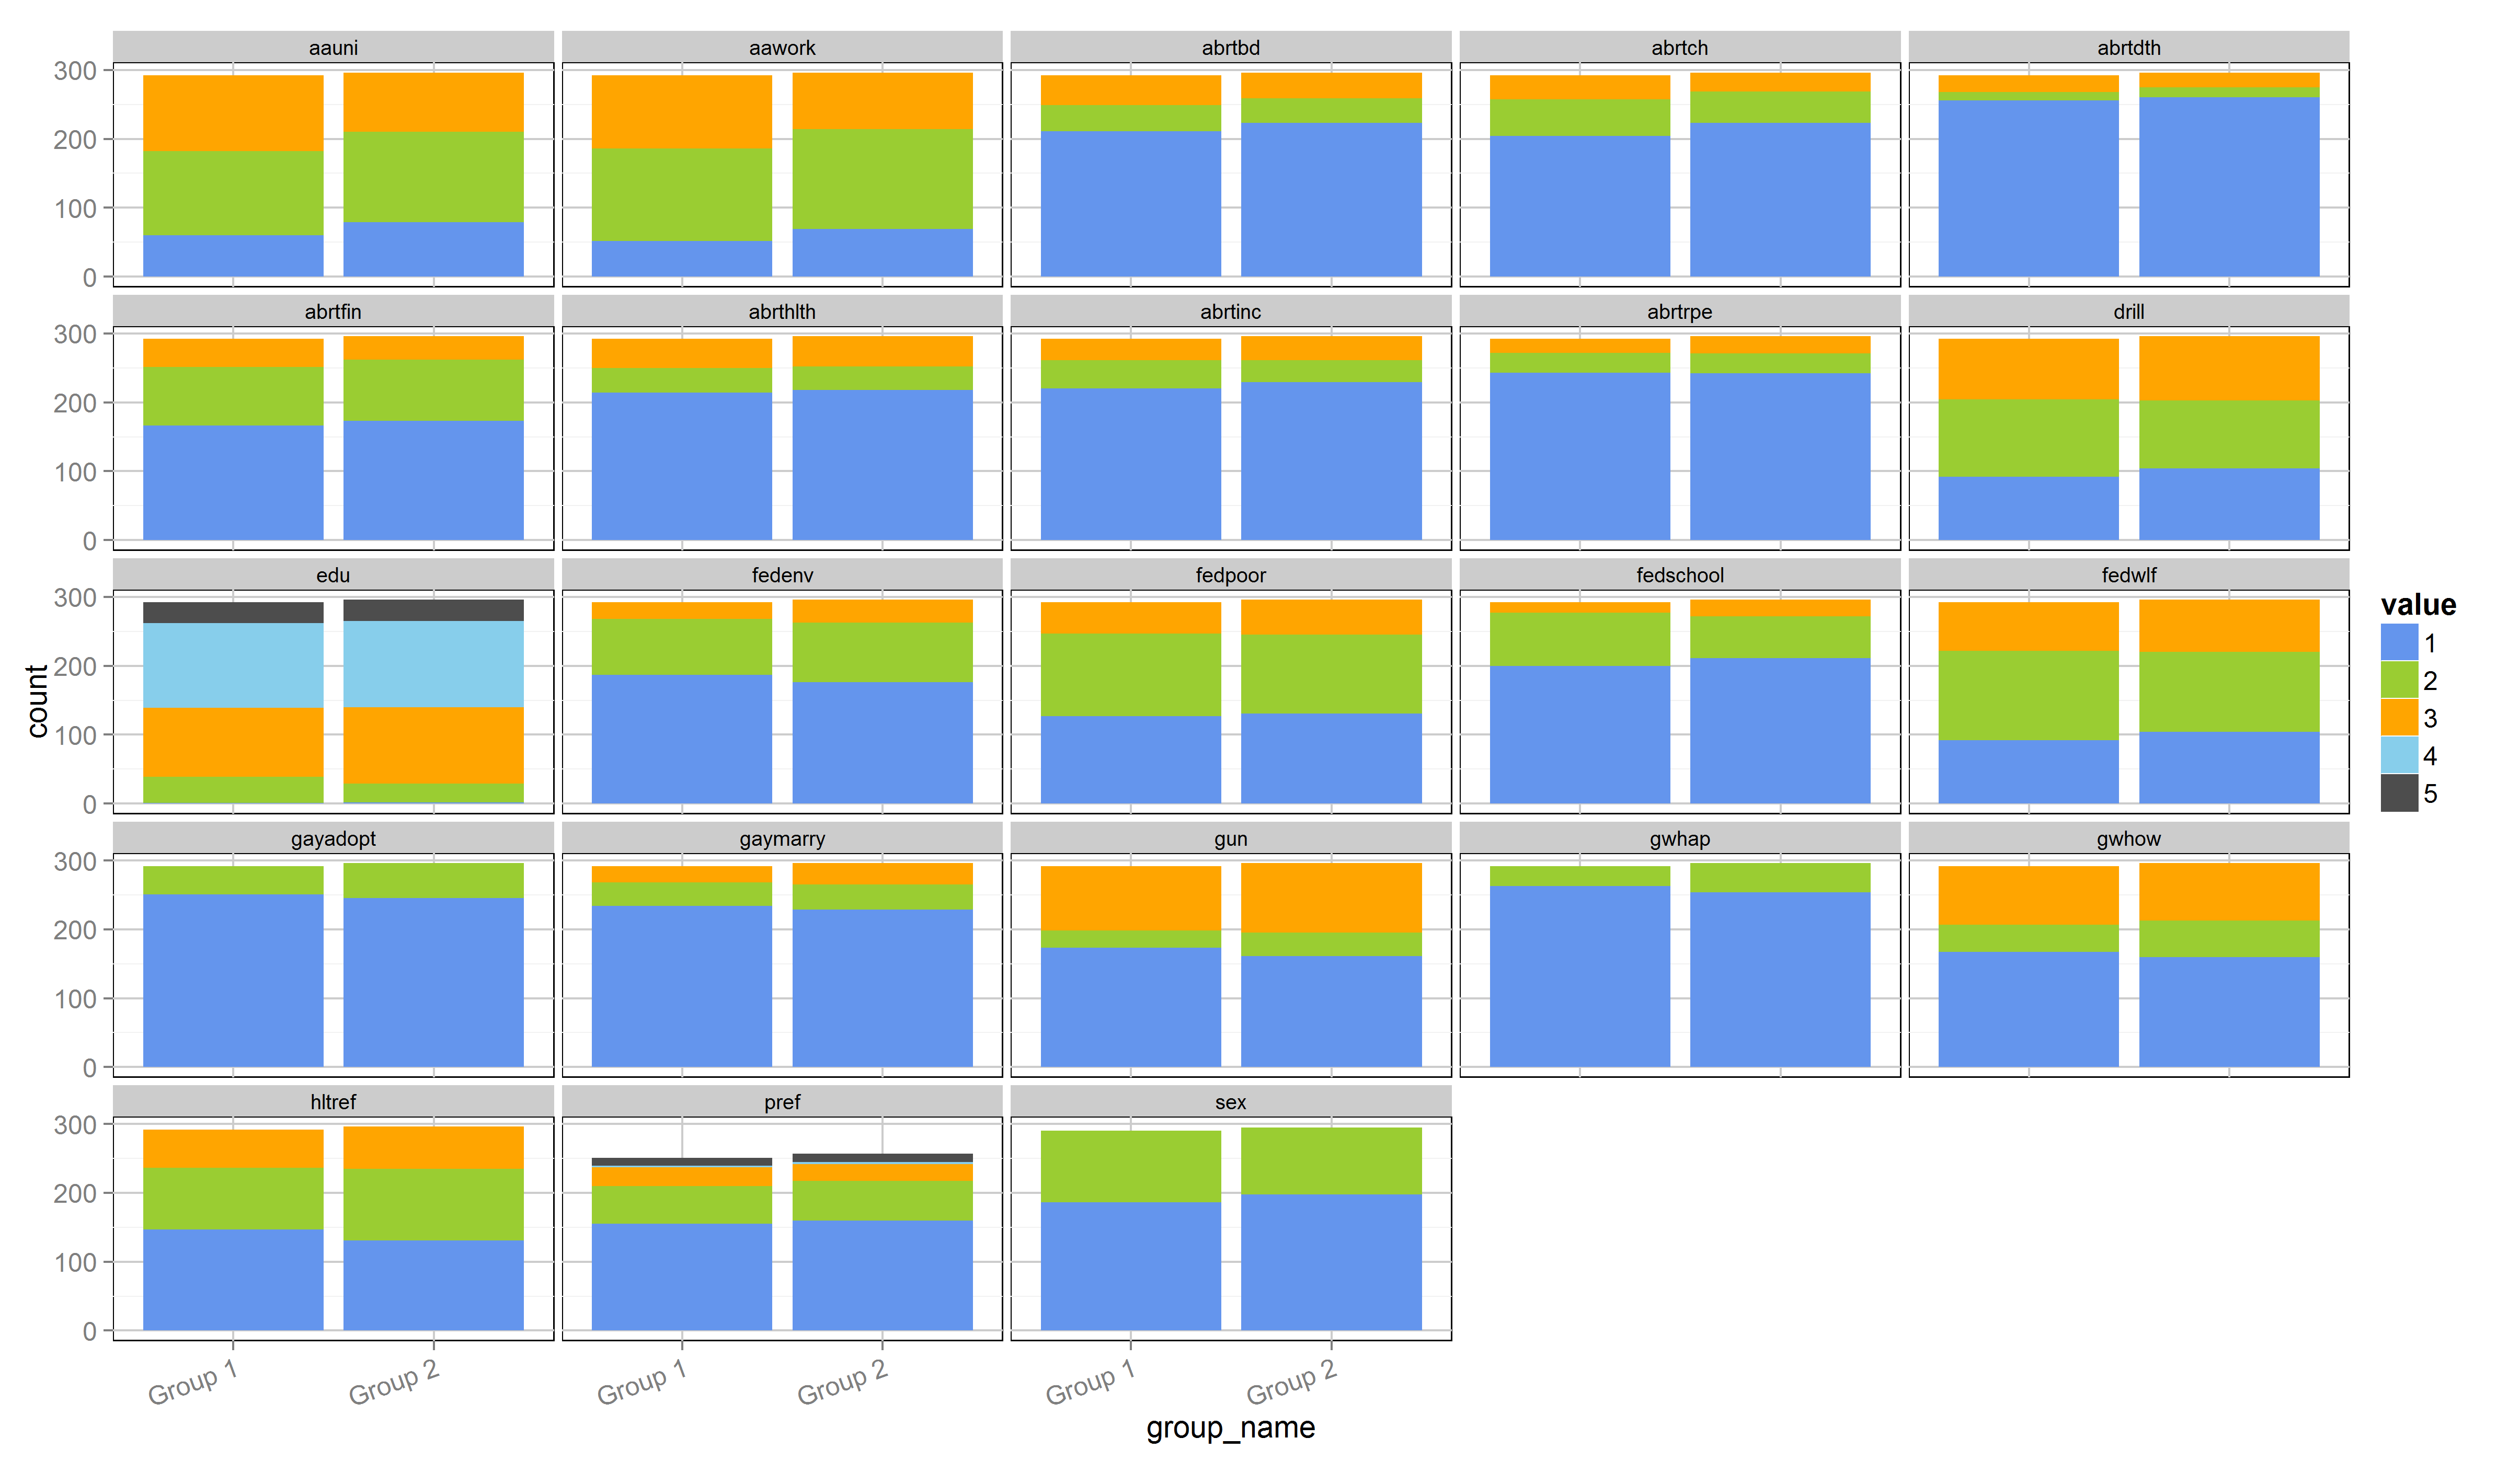
\includegraphics{../figures/main/bal.png}
  \caption{Balance of answers to issue questions in the survey group. Full variable names can be found in Table \ref{tab:predictors}}
  \label{fig:bal}
\end{figure}

\begin{figure}[ht!]
  \centering
  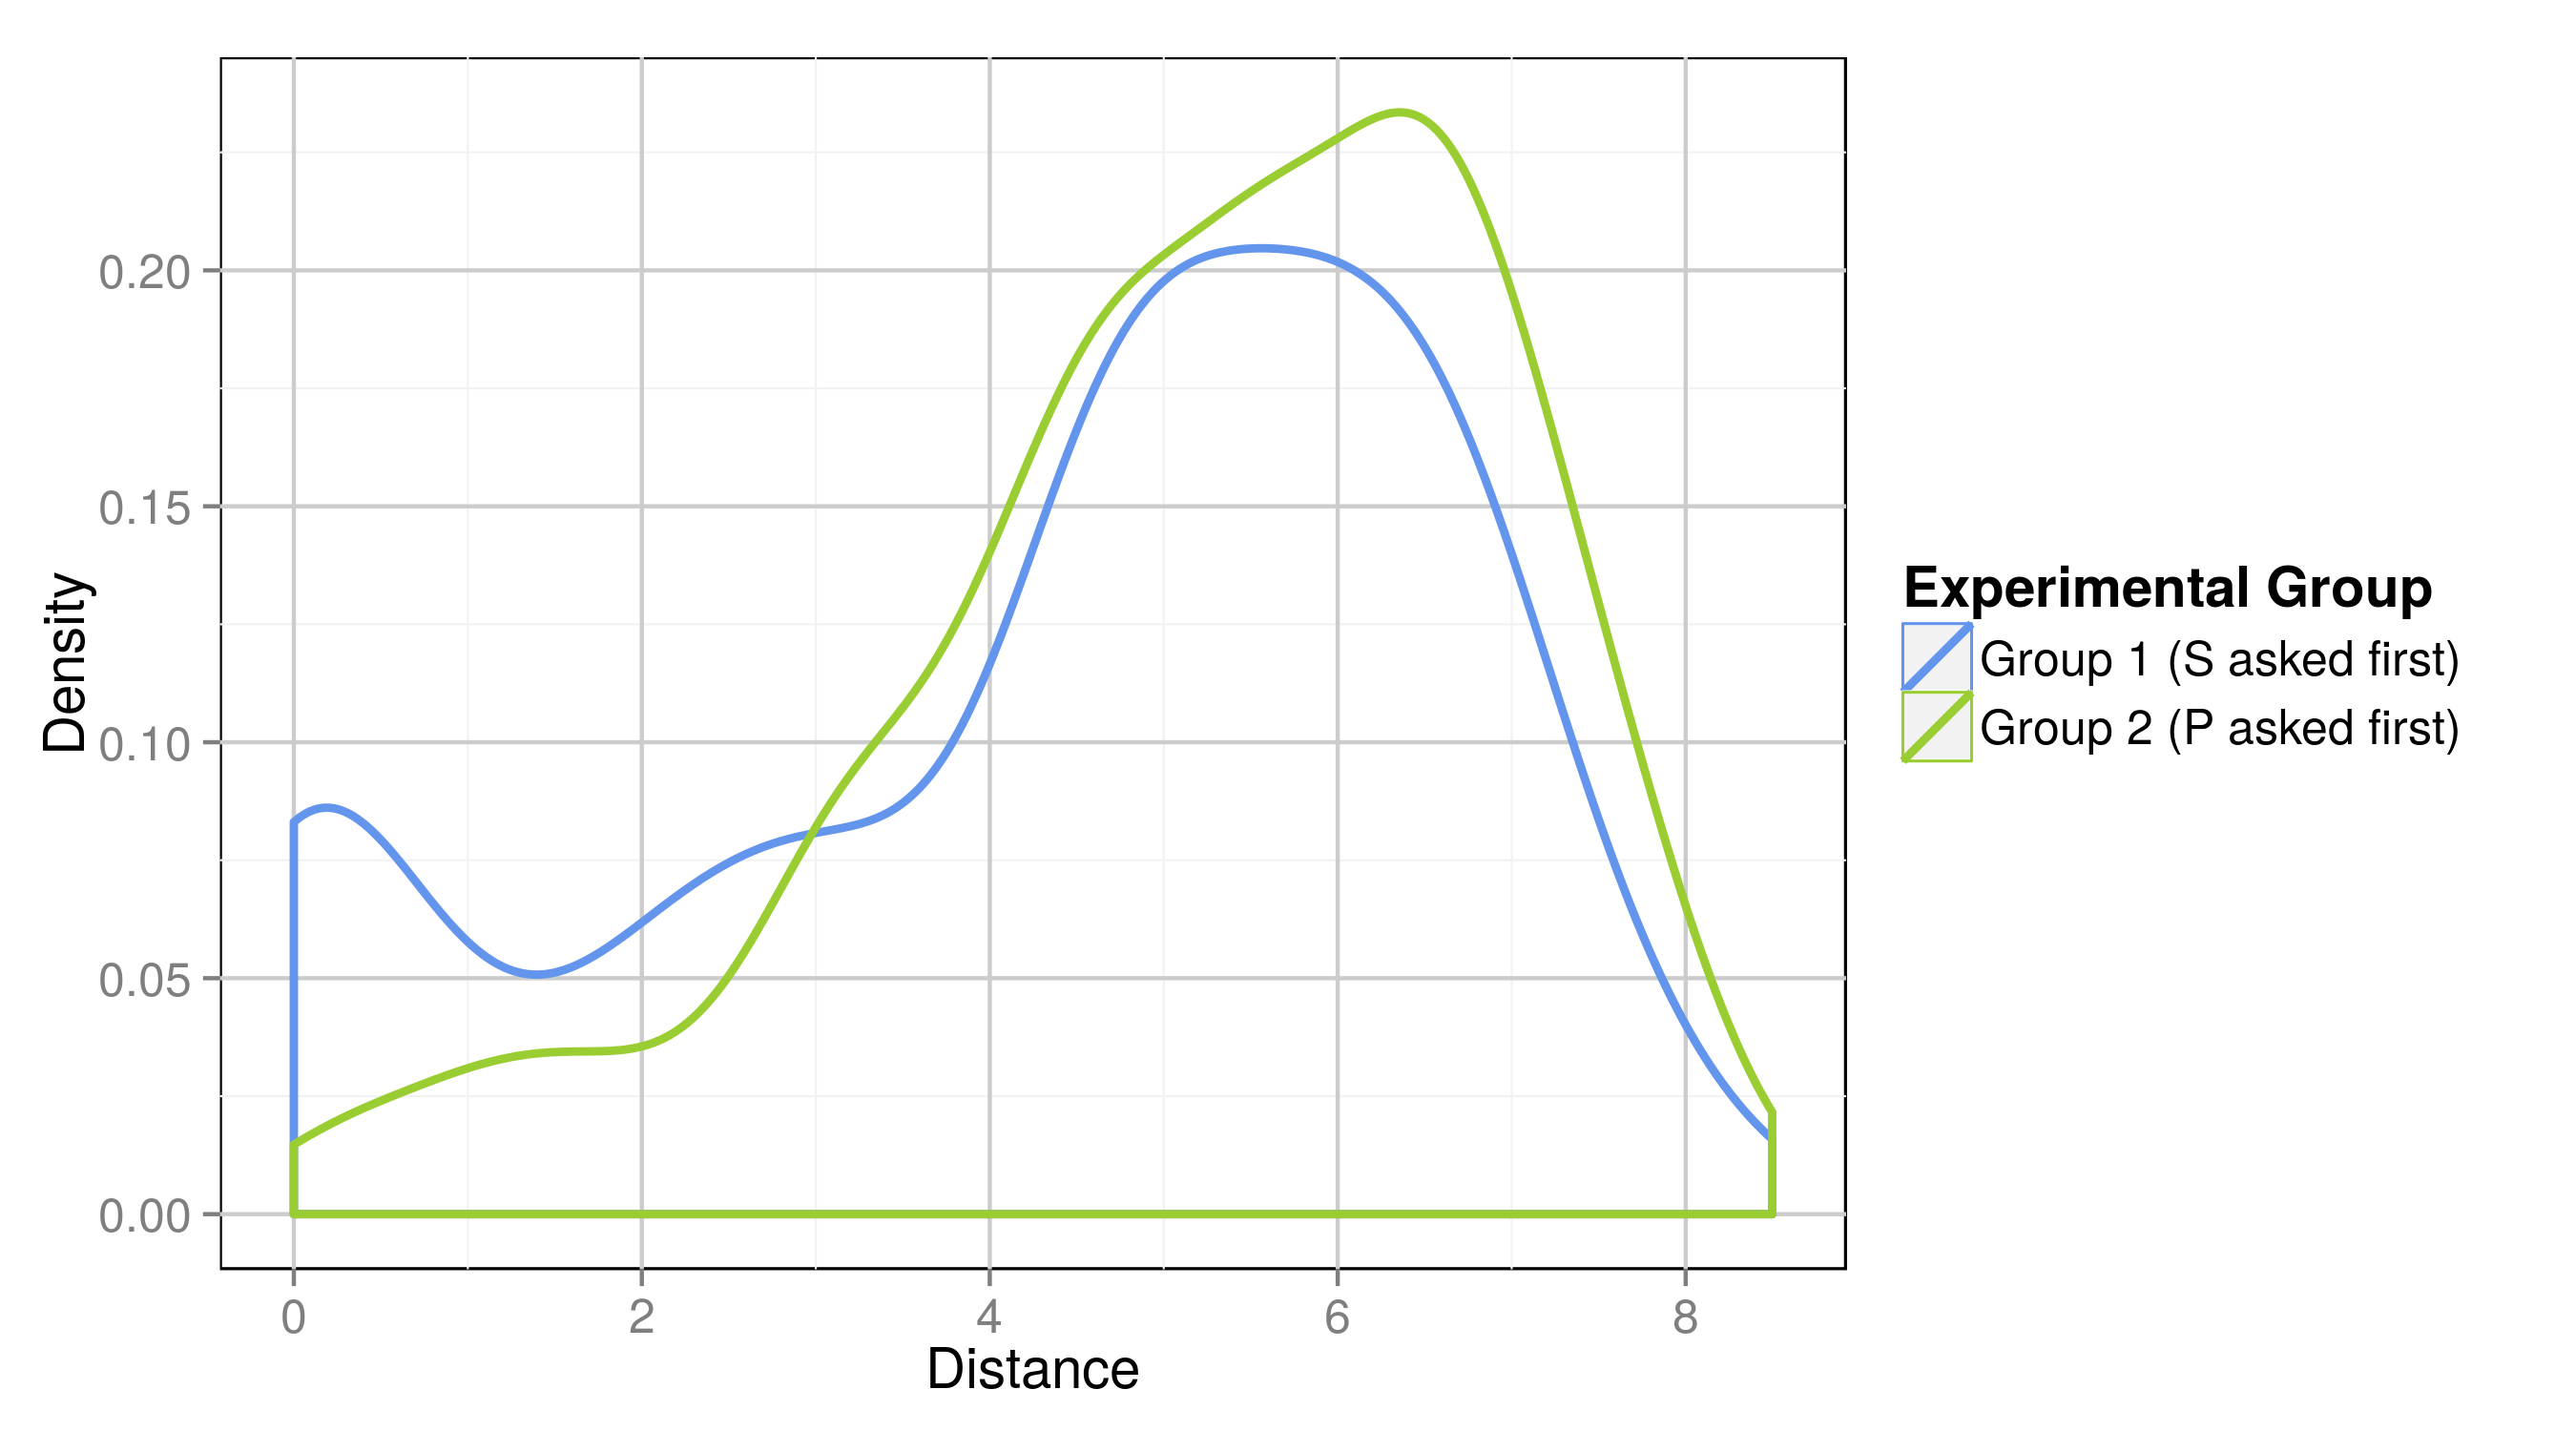
\includegraphics{../figures/main/dist_dista_log.png}
  \caption{Distribution of logarithmic transformation of distances for Experiment 2. The following transformations have been applied: $Z_t = ln(Z + 1)$ (Blue line) and $W_t = ln(W + 1)$ (Green line).}
  \label{fig:d_dist_log}
\end{figure}

% latex table generated in R 3.1.3 by xtable 1.7-4 package
% Thu Apr  2 17:50:24 2015
\begin{table}[ht]
\centering
\begin{tabular}{lrr}
  \hline
 & Statistic & p-value \\ 
  \hline
X & 0.609 & 0.000 \\ 
  Y & 0.702 & 0.000 \\ 
  log(Z + 1) & 0.814 & 0.000 \\ 
  log(W + 1) & 0.930 & 0.000 \\ 
   \hline
\end{tabular}
\caption{Kolmogorov-Smirnoff test for normality
                 for the outcomes of Experiment 1 and the log-transformed outcomes of
                 Experiment 2. In all cases the Null-Hypothesis of a normal distribution
                 is rejected} 
\label{tab:ks}
\end{table}


\clearpage

\subsection{Predictive Model}

\begin{figure}[ht!]
  \centering
  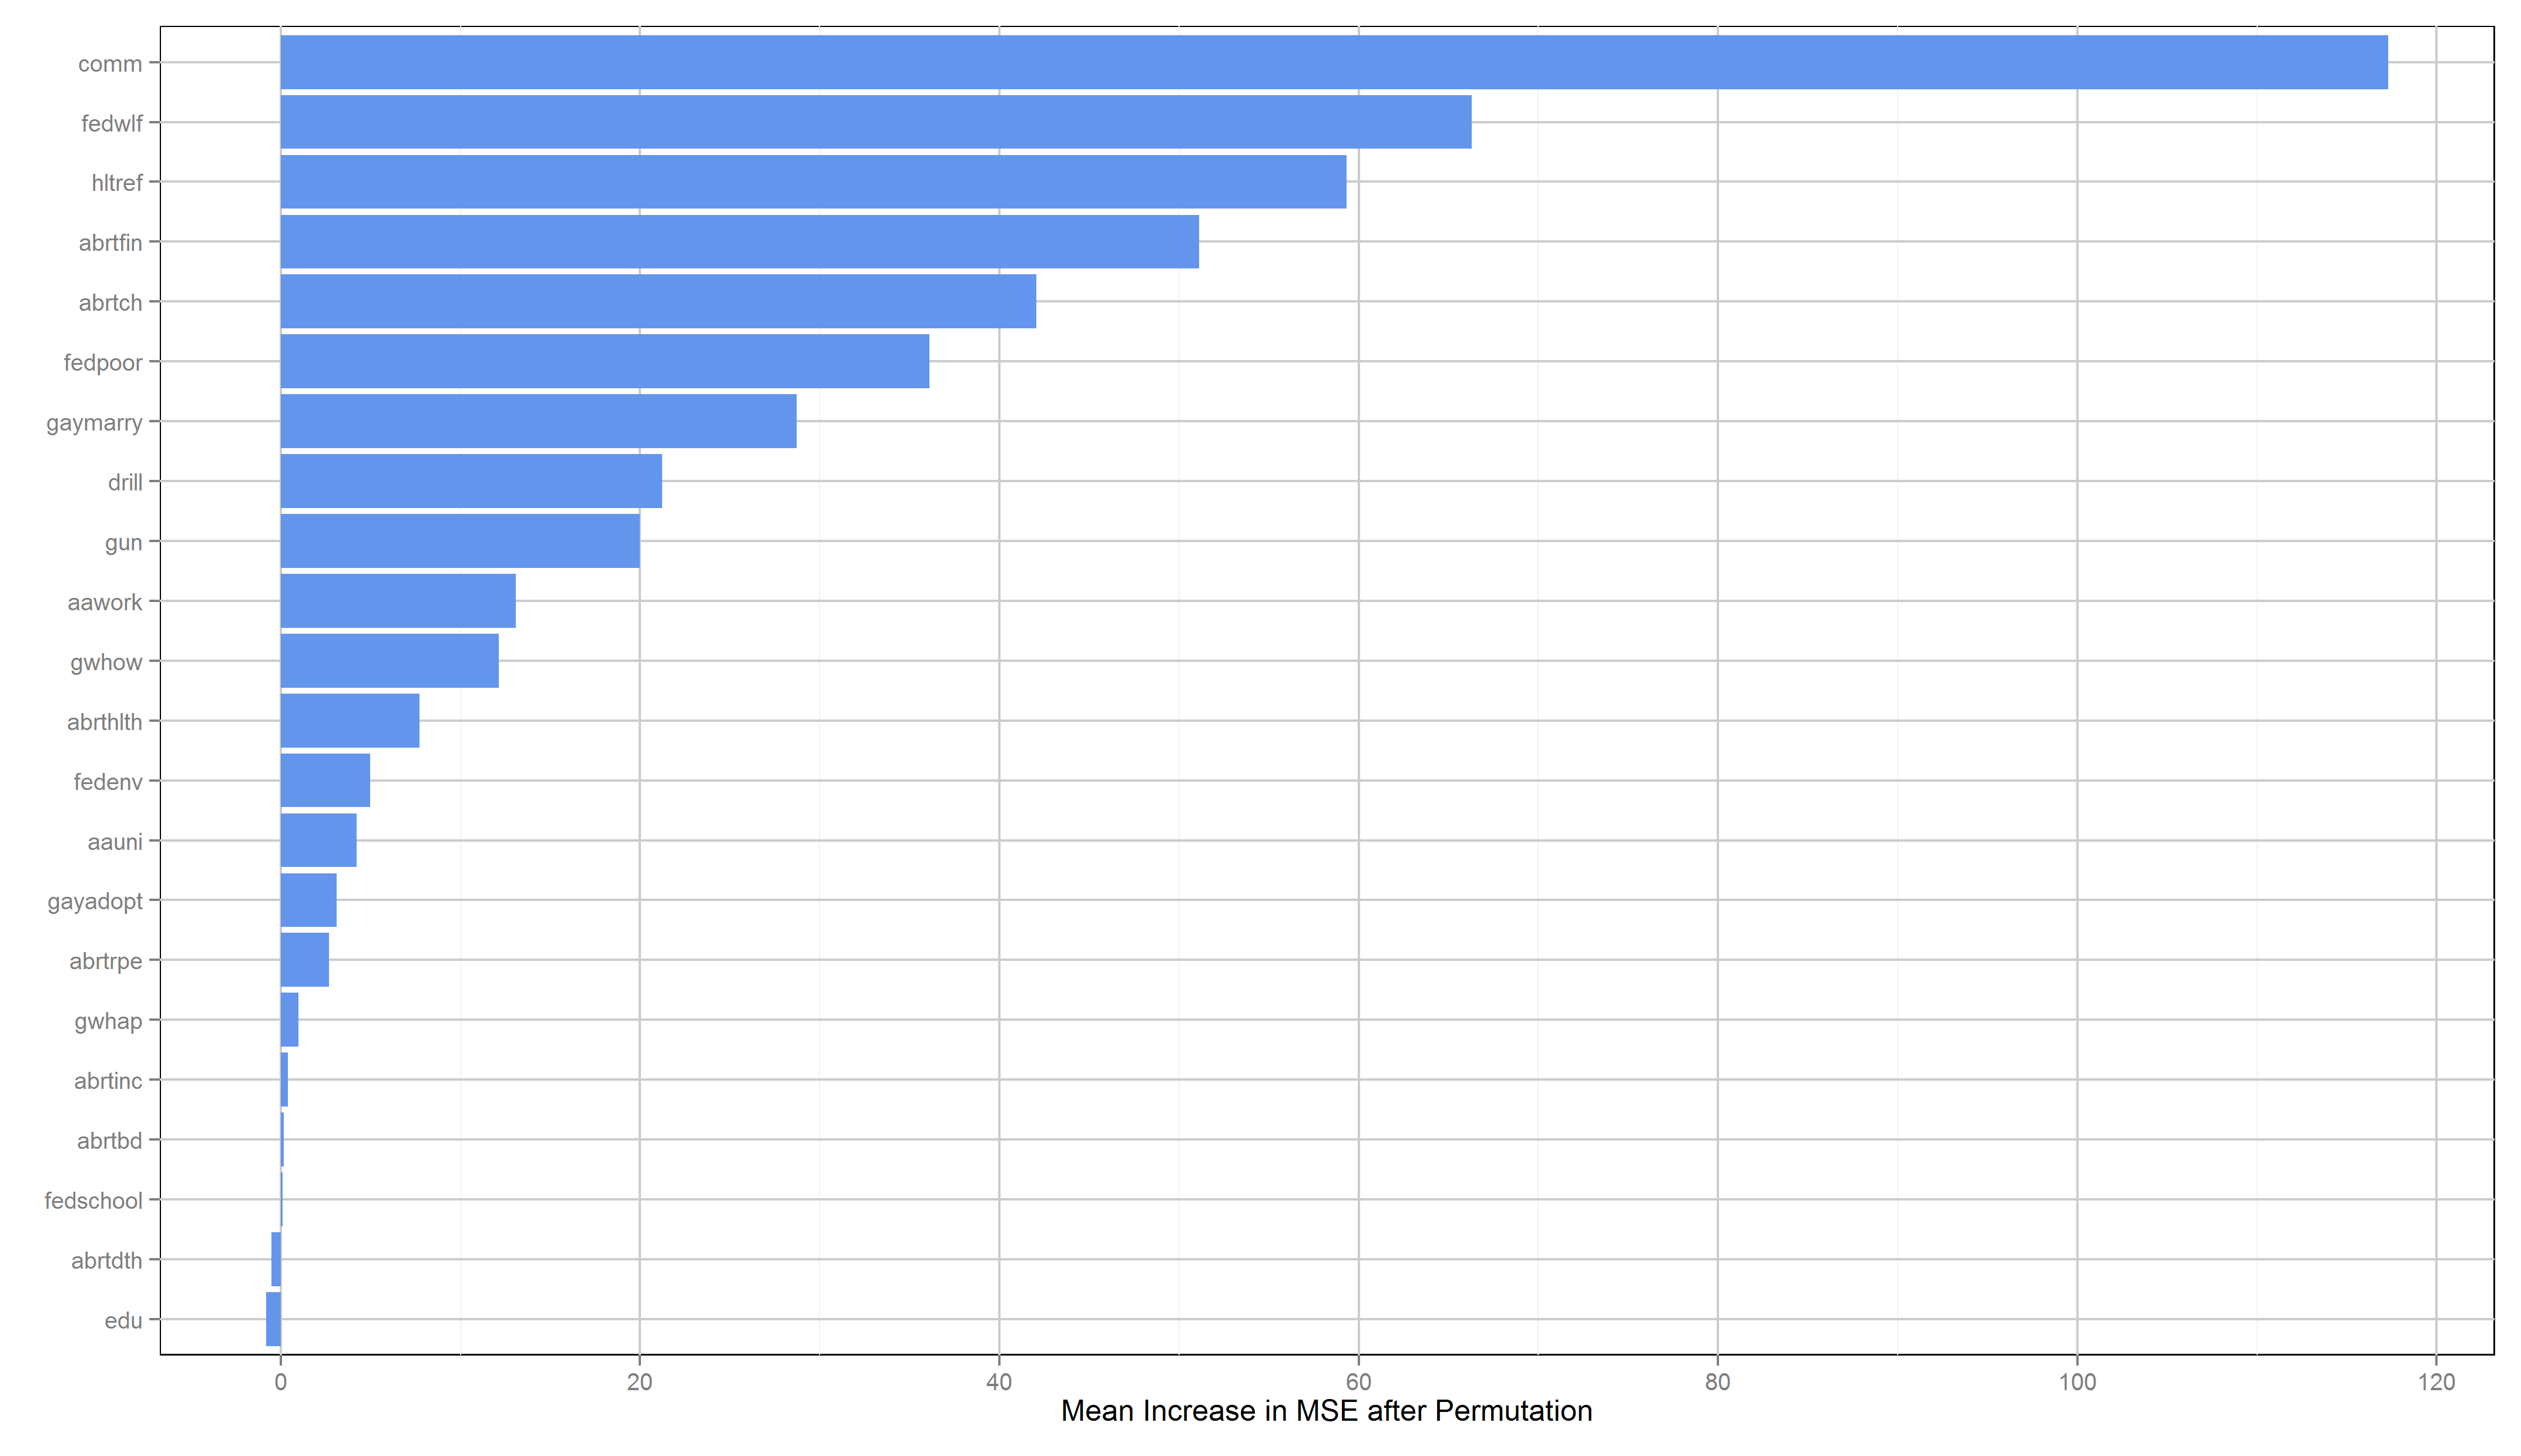
\includegraphics{../figures/main/varimp.png}
  \caption{Permutation importance of predictors in random forest model. Meanings of the variable abbreviatiosn can be found in Table \ref{tab:predictors}.}
  \label{fig:imp}
\end{figure}

\begin{figure}[ht!]
  \centering
  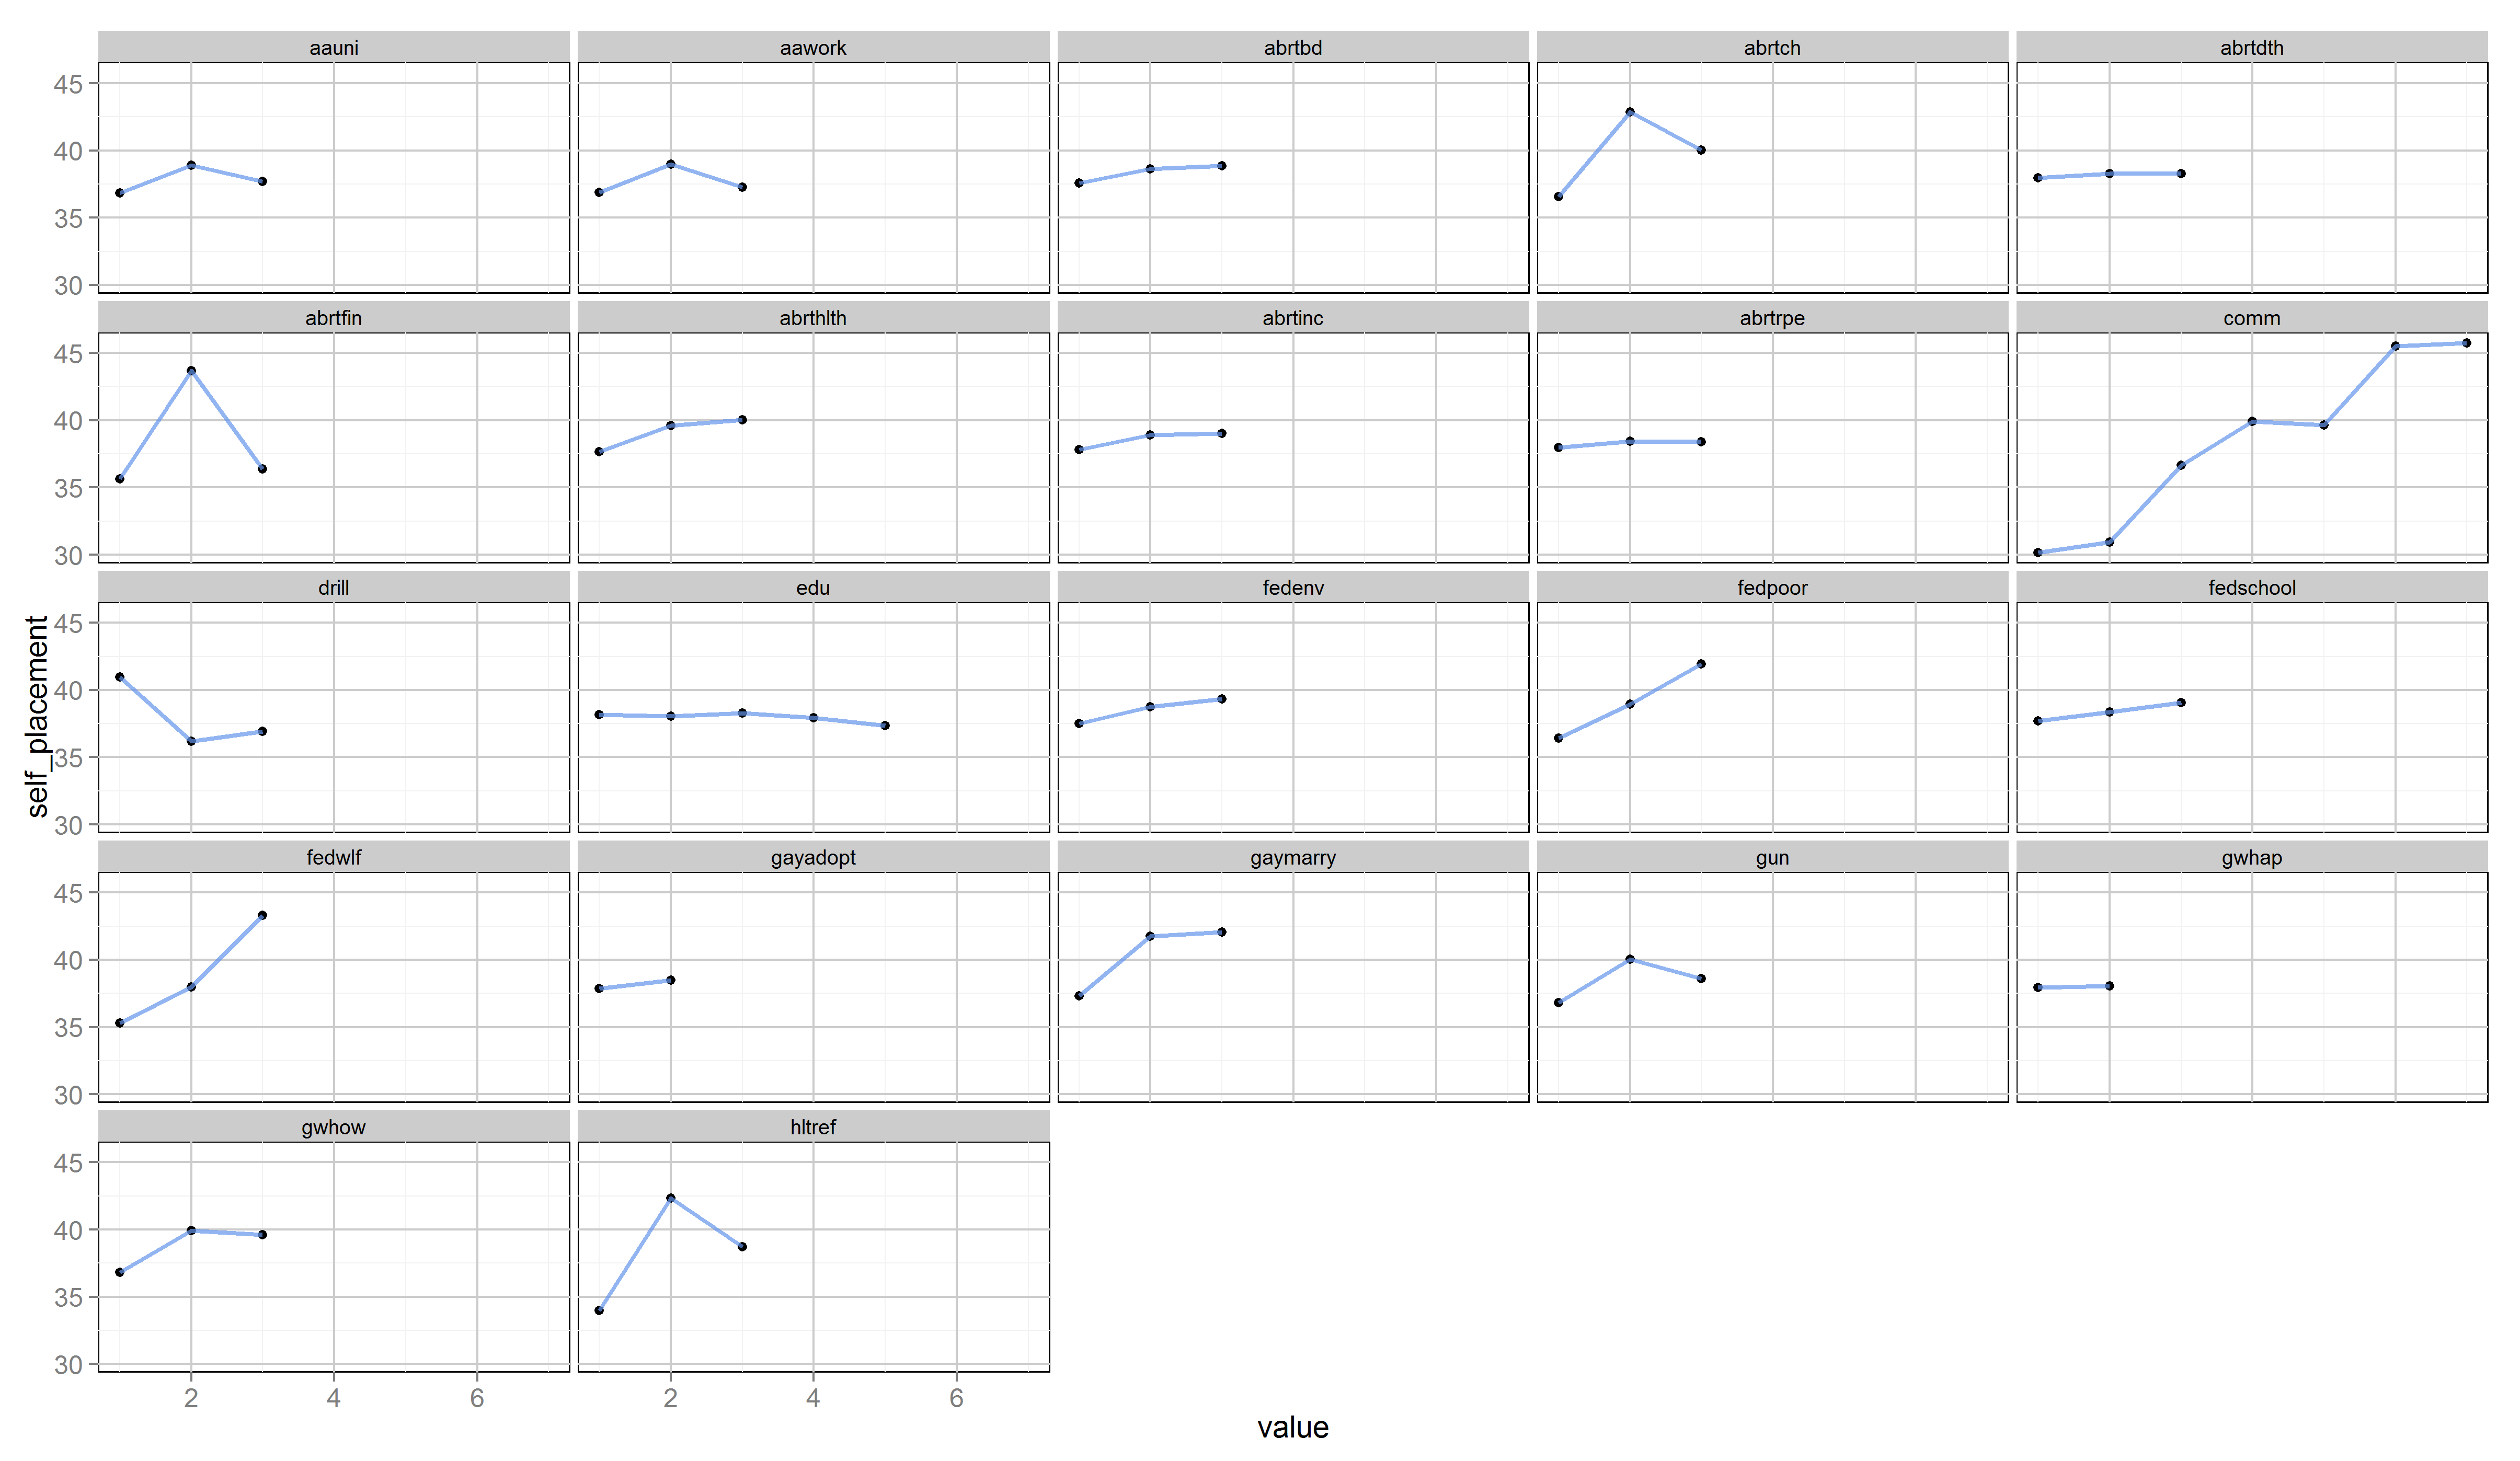
\includegraphics{../figures/main/partial_dependence.png}
  \caption{Partial dependence for predictor variables. Variable abbreviations and codings can be found in Table \ref{tab:predictors}.}
  \label{fig:pd}
\end{figure}

\begin{table}[ht]
\centering
\begin{tabular}{lllll}
\hline
Variable  & Question                                   & 1                                      & 2             & 3             \\
\hline
hltref    & Health care reform 2010                    & Favor                                  & Oppose        & Neither       \\
abrtch    & Abortion if the woman chooses              & Favor                                  & Oppose        & Neither       \\
gaymarry  & Gay marriage                               & Favor                                  & Oppose        & Neither       \\
gayadopt  & Gay couples adopting children              & Favor                                  & Oppose        & Neither       \\
abrthlth  & Abortion if pregnancy harms  health        & Favor                                  & Oppose        & Neither       \\
abrtinc   & Abortion if pregnancy from incest          & Favor                                  & Oppose        & Neither       \\
abrtbd    & Abortion if child has a birth defect       & Favor                                  & Oppose        & Neither       \\
fedwlf    & Federal welfare spending                   & Increase                               & Keep the same & Decrease      \\
abrtfin   & Abortion for financial reasons             & Favor                                  & Oppose        & Neither       \\
abrtrpe   & Abortion after rape                        & Favor                                  & Oppose        & Neither       \\
fedpoor   & federal spending on poor                   & Increase                               & Keep the same & Decrease      \\
fedenv    & Federal spending for environment           & Increase                               & Keep the same & Decrease      \\
fedschool & Federal spending on public schools         & Increase                               & Keep the same & Decrease      \\
drill     & Offshore drilling                          & Favor                                  & Oppose        & Neither       \\
gwhap     & Global warming happening                   & Yes                                    & No            &               \\
gwhow     & Cause for global warming                   & Human                                  & Natural       & Both          \\
aauni     & Affirmative action university              & Favor                                  & Oppose        & Neither       \\
aawork    & Affirmative action workplace               & Favor                                  & Oppose        & Neither       \\
gun       & Access to guns should be                   & More difficult                         & Easier        & Keep the same \\
comm      & Government or self responsibility          & Scale from   							&  1        to  &   7           \\
\hline
\end{tabular}
\caption{Abbreviations and coding of predictors in random forest model. See the online appendix for the full wording of the questions and the full survey.}
\end{table}

\clearpage

\subsection{Frequentist Test}

% latex table generated in R 3.1.3 by xtable 1.7-4 package
% Thu Apr  2 16:59:03 2015
\begin{table}[ht]
\centering
\begin{tabular}{rrr}
  \hline
 & Experiment 1 & Experiment 2 \\ 
  \hline
Statistic & 29238.000 & 26497.000 \\ 
  p-value & 0.034 & 0.000 \\ 
   \hline
\end{tabular}
\caption{Wilcoxon rank tests for Experiments 1
             and 2. P-values for one sided tests.} 
\label{tab:np_res}
\end{table}


% latex table generated in R 3.1.3 by xtable 1.7-4 package
% Thu Apr  2 17:08:38 2015
\begin{table}[ht]
\centering
\begin{tabular}{rrrrr}
  \hline
 & Group 1 (control) & Group 2 & Difference in Means & p-value \\ 
  \hline
 & 7.923 & 10.795 & -2.872 & 0.053 \\ 
   \hline
\end{tabular}
\caption{One sided T-test for Experiment 1} 
\label{tab:ttest}
\end{table}


\clearpage

%\subsection{MCMC Diagnostics}

%\begin{figure}[ht!]
%  \centering
%  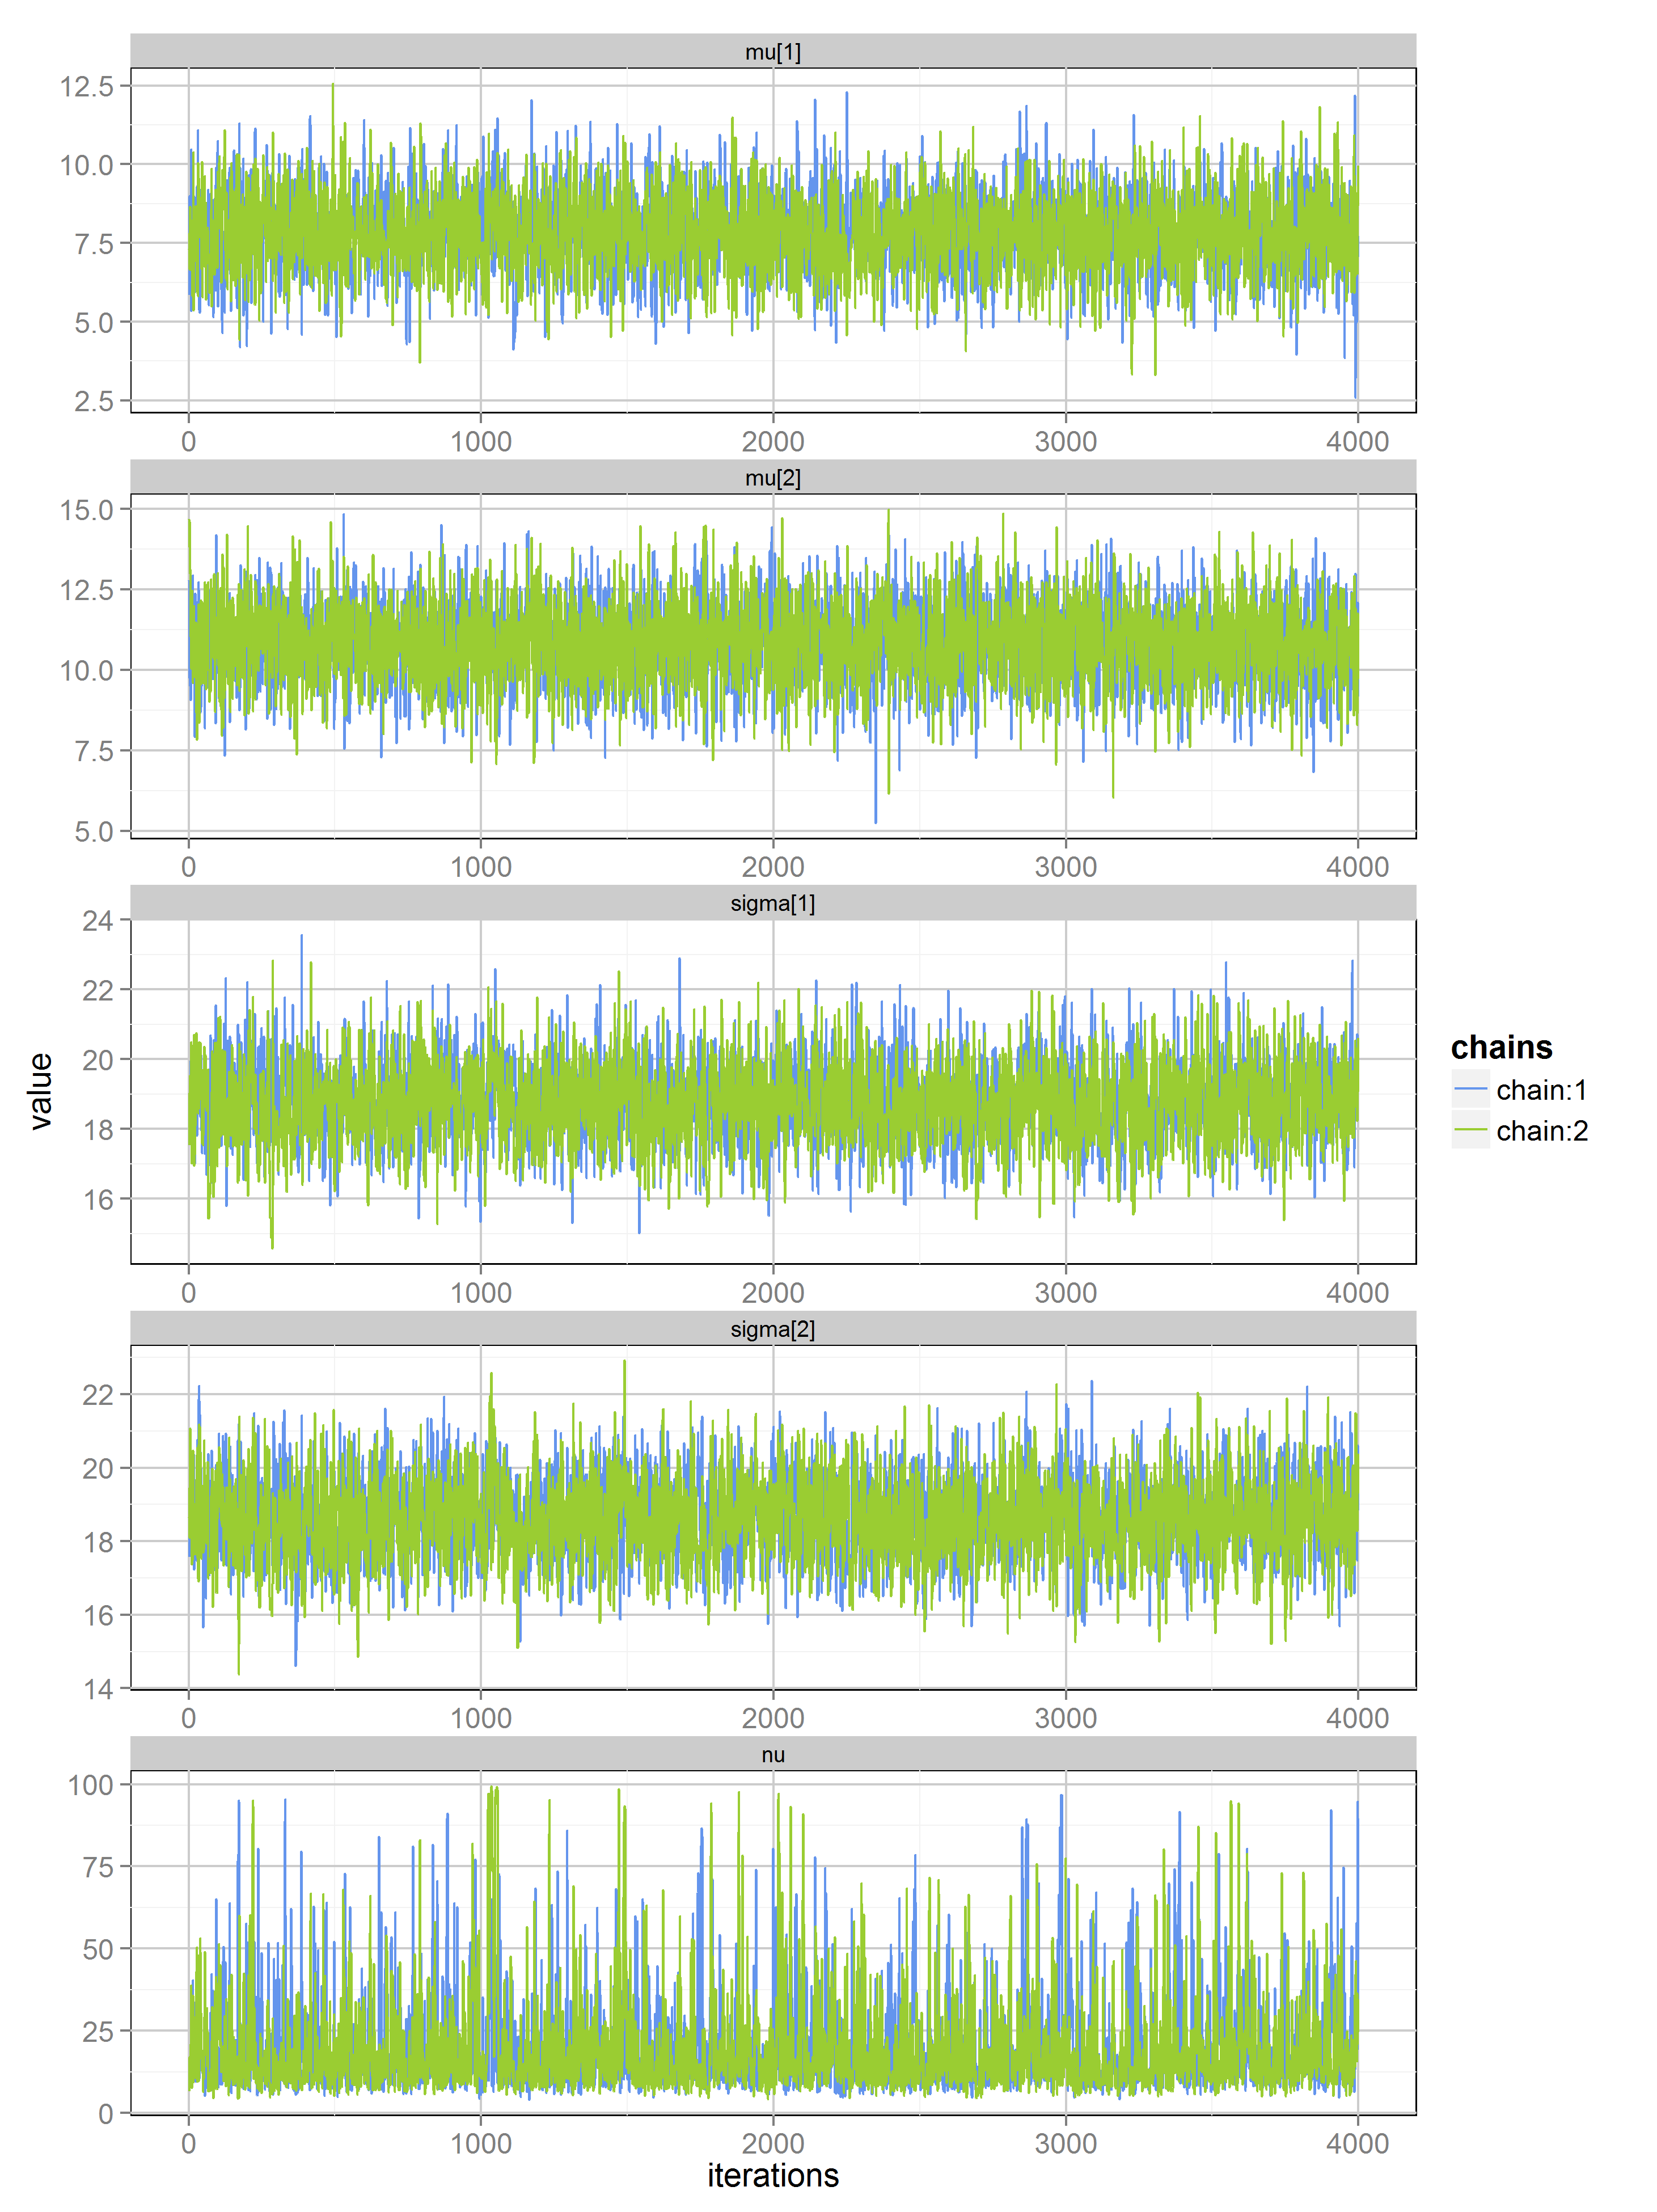
\includegraphics{../figures/main/trace_1.png}
%  \caption{Traceplots for parameters in Experiment 1.}
%  \label{fig:trace_1}
%\end{figure}

%\begin{figure}[ht!]
%  \centering
%  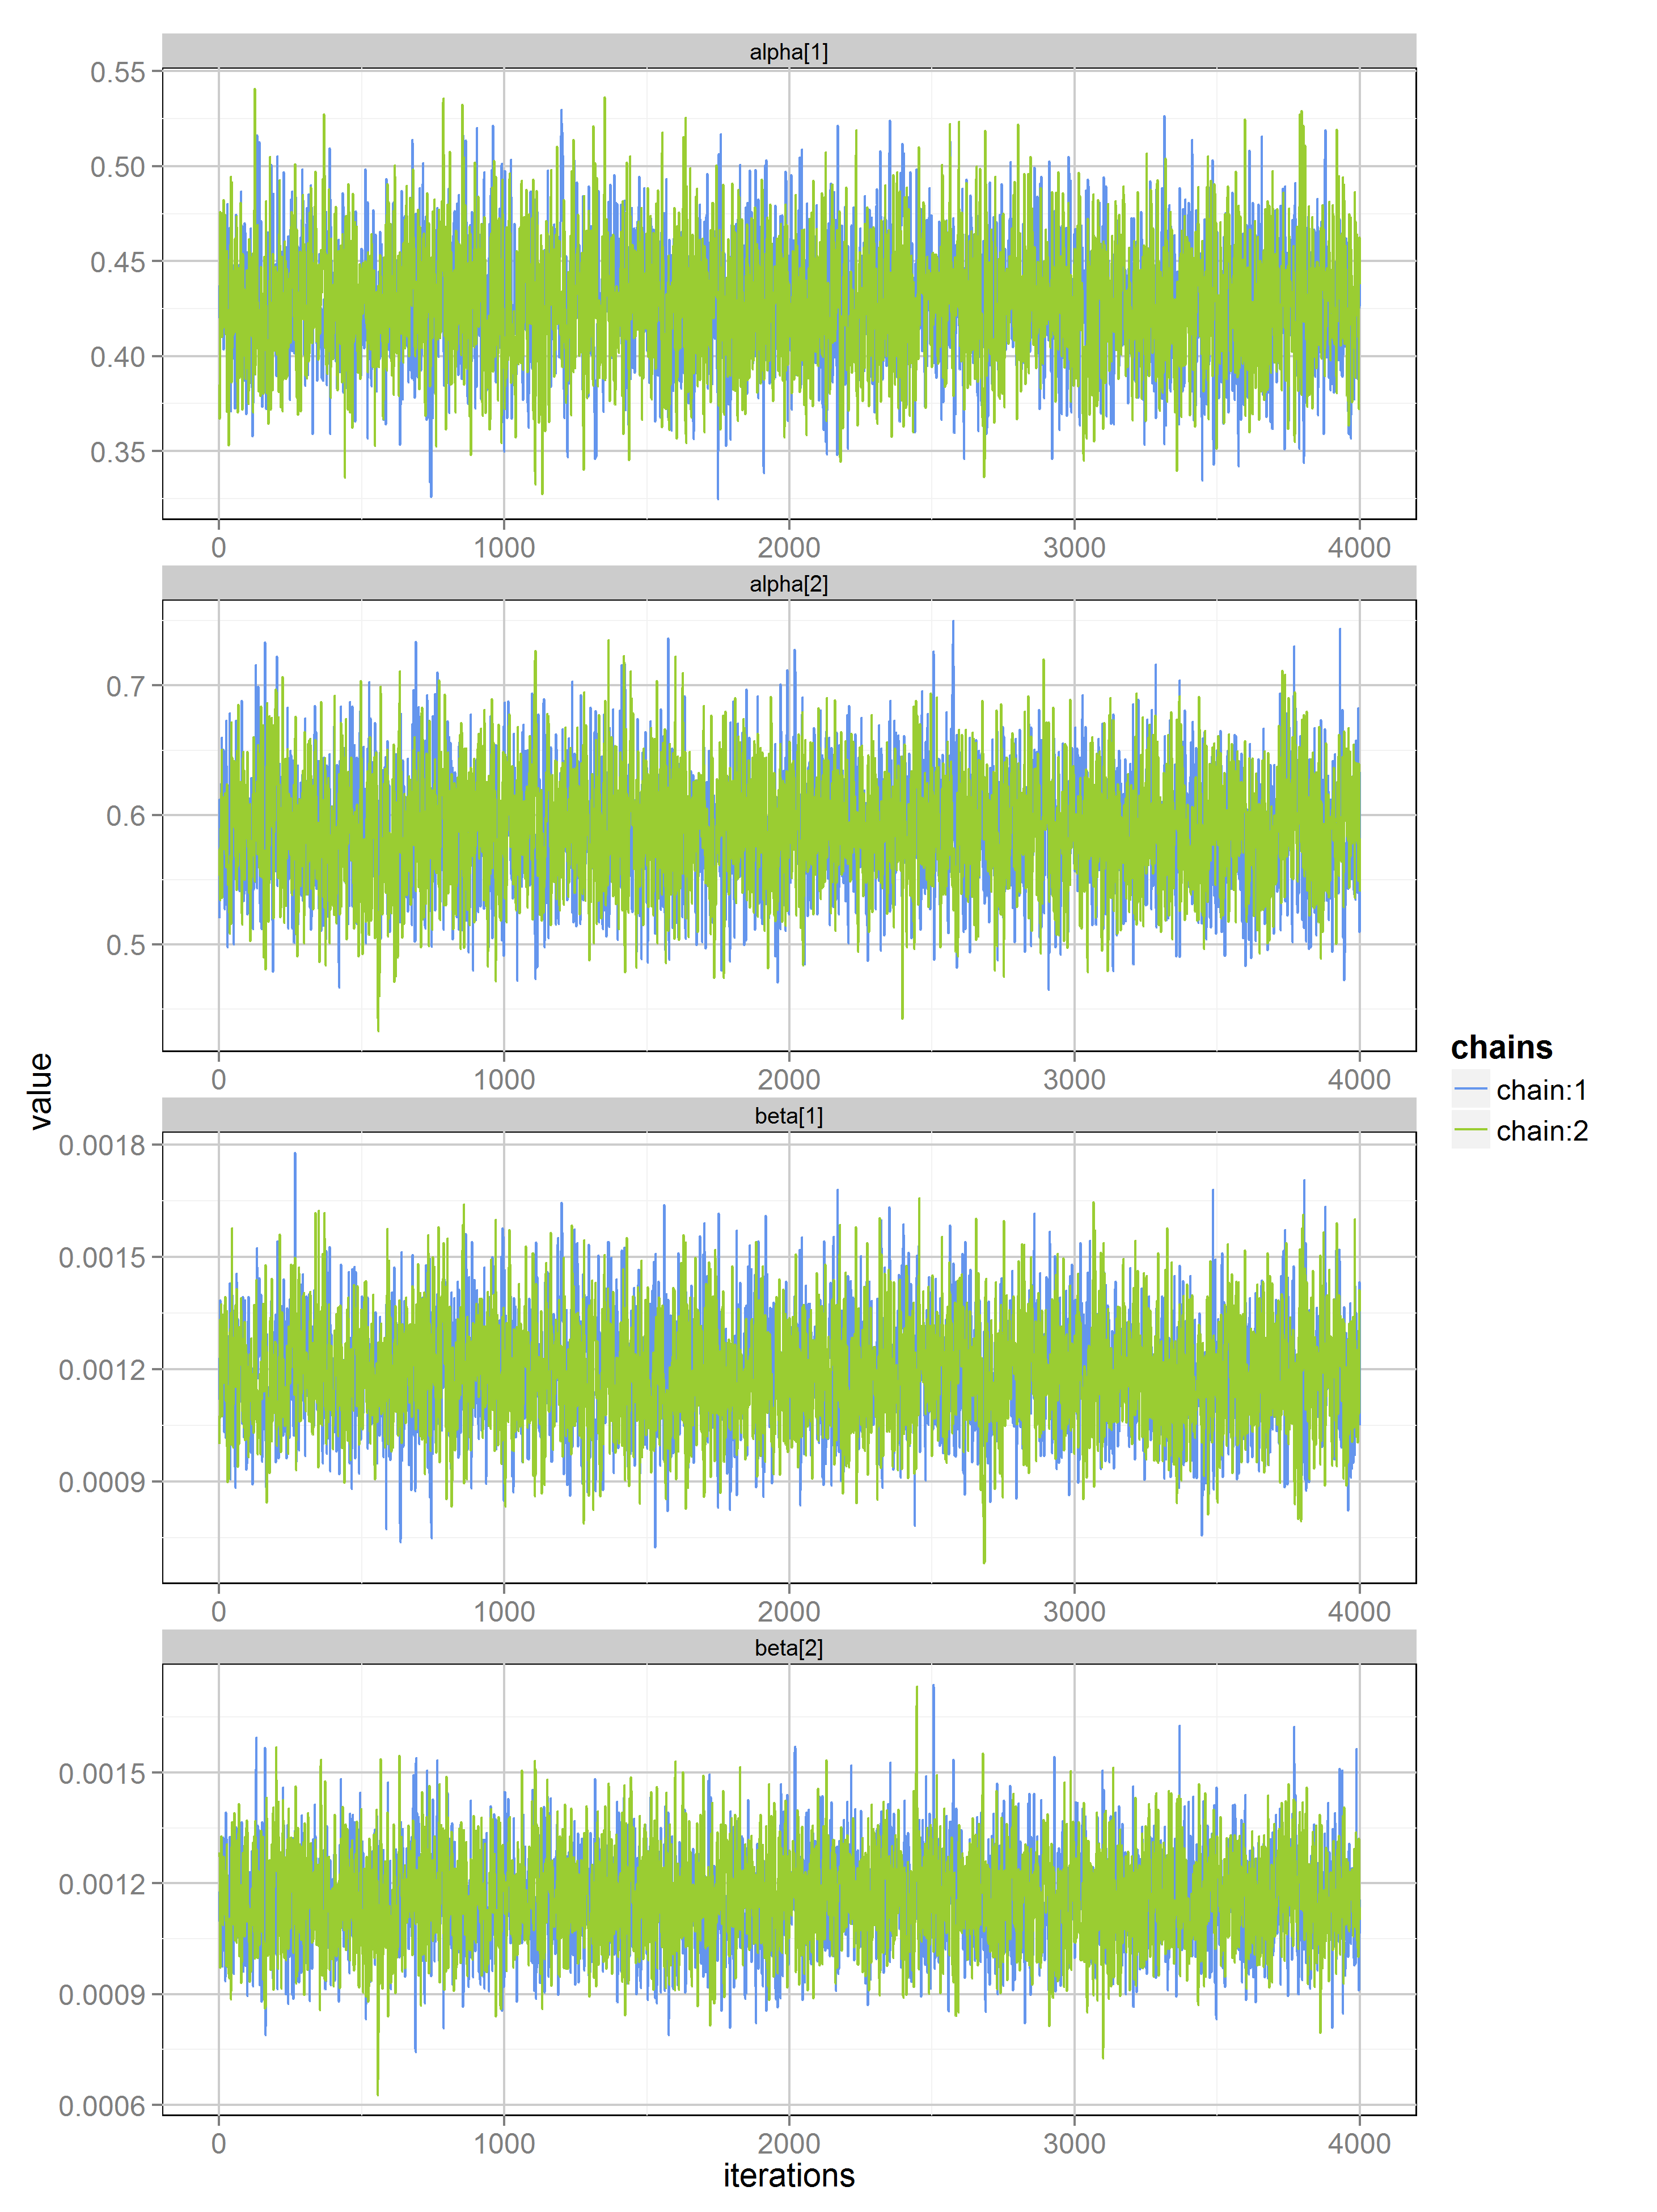
\includegraphics{../figures/main/trace_2.png}
%  \caption{Traceplots for parameters in Experiment 2.}
%  \label{fig:trace_2}
%\end{figure}
